\section{Struktura modela neuronske mreže}

Principi strukturiranja konvolucijske neuronske mreže za klasifikaciju matričnih podataka
poput upravo pripremljenih prate opis u poglavlju o CNN-ovima \ref{sec:cnn}.
Uz to, postoji zahtjev za što manjim modelom jer ga je potrebno implementirati na 
mikrokontrolerskoj platformi koja ima ograničavajuće memorijske resurse. Također,
vrijeme potrebno za buđenje neuronske mreže, tj. kašnjenje koje unosi mreža
implementirana na mikrokontroleru izravno utječe na performanse sustava 
koji bi trebao raditi u stvarnom vremenu. Imajući to na umu, izgrađena
mreža bit će dovoljno jednostavna da zadovolji spomenute uvjete, a s druge strane dovoljno
složena, tako da je sposobna pravilno klasificirati ulazne podatke.

Ulazni podaci su matrice dimenzija (32, 41, 12, 1). Podmatrica dimenzija (41, 12) 
predstavlja matricu značajki pojedinog zvučnog zapisa. U konfiguraciji je odabrano 
12 MFC koeficijenata (od 2. do 13.), a zbog veličine prozora (\texttt{WINDOW\_SIZE}) 
koja iznosi 512 (32 ms) i veličine koraka (\texttt{STEP\_SIZE}) koja iznosi 384 (24 ms)
jedna sekunda zapisa se sastoji od 41 vremenskog okvira. Dodatne dimenzije matrice
predstavljaju redom broj takvih matrica koje se odjednom daju mreži na treniranje 
(\texttt{BATCH\_SIZE}) te dimenzija slike koja u ovom slučaju iznosi jedan. Konvolucijske
neuronske mreže također mogu raditi s višekanalnim matricama kao što su RGB slike. U tom 
slučaju svaki kanal predstavlja prisutnost određene boje u slici. Matrice značajki
generirane nad zvučnim zapisima ponašaju se kao crno-bijele slike gdje svaka vrijednost
predstavlja svjetlinu određenog piksela.

Ulazni sloj u neuronsku mrežu prate dva konvolucijska s pripadnim slojevima za
poduzorkovanje. Prvi konvolucijski sloj ima 32 jezgre veličine \texttt{3x3},
a drugi njih 16 iste veličine. Oba sloja za poduzorkovanje rade s matricom
veličine \texttt{2x2} te pomakom iznosa dva. Slijedi ih podmreža koja se sastoji 
od dva potpuno povezana sloja 
s, redom, 8 i 16 neurona te izlazni sloj koji ima točno 7 neurona (svaki za jednu
klasifikacijsku kategoriju). Aktivacije svih slojeva su "ReLu", dok izlazni sloj
koristi "softmax" aktivaciju. Isječak koda \ref{code:network} prikazuje postupak
izgradnje opisane mreže.

\begin{lstlisting}[language=C++, caption=Struktura mreže, label=code:network]
model = tf.keras.Sequential([
    layers.Input(shape=input_shape),    # Input layer
    layers.Conv2D(32, kernel_size=3, padding='same', activation='relu'),
    layers.MaxPooling2D(pool_size=2, strides=2, padding='same'),
    layers.Conv2D(16, kernel_size=3, padding='same', activation='relu'),
    layers.MaxPooling2D(pool_size=2, strides=2, padding='same'),
    layers.Flatten(),   # Flatten the data for fully connected layers
    layers.Dense(8, activation='relu'),   # Fully connected layer
    layers.Dropout(0.1),                  # Dropout layer with 10% rate
    layers.Dense(16, activation='relu'),  # Fully connected layer
    layers.Dropout(0.1),                  # Dropout layer with 10% rate
    layers.Dense(num_labels, 'softmax'),  # Output layer (softmax)
])
\end{lstlisting}

Na slici \ref{pic:struktura} prikazan je model neuronske mreže s pripadnim brojem
parametara te oblikom podataka između slojeva. Oblik podataka ima prvu dimenziju 
neodređenu (na slici "?") zbog toga što se mreža može trenirati s proizvoljnom 
veličinom grupe (brojem uzoraka koji se odjednom daju mreži).

\begin{figure}[htb]
    \centering
    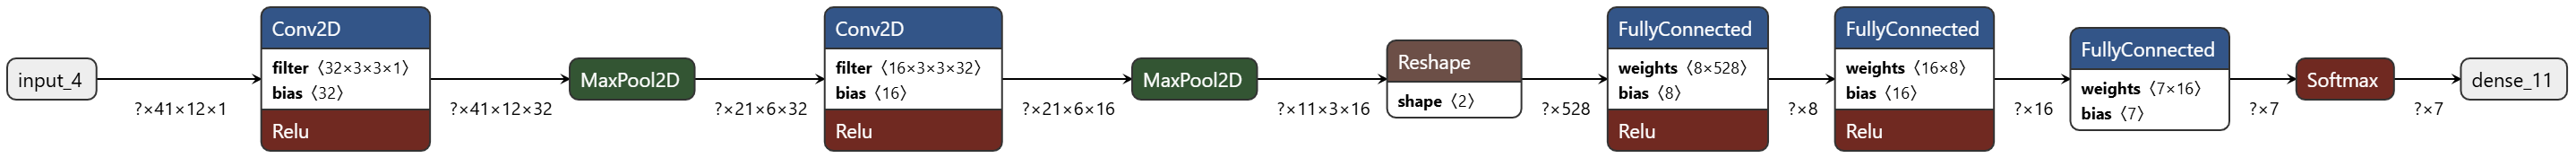
\includegraphics[width=1\linewidth]{Chapters/neuronska_mreza/struktura/model.png} 
    \caption{Neuronska mreža \cite{netron}}
    \label{pic:struktura}
\end{figure}

